\documentclass[acmlarge,nonacm]{acmart}

% Journal metadata
\acmJournal{TQC}

% Additional packages (acmart already loads amsmath, amssymb, graphicx, hyperref)
\usepackage{booktabs}
\usepackage{siunitx}
\usepackage{algorithm}
\usepackage{algpseudocode}

% Custom commands
\newcommand{\ket}[1]{|#1\rangle}
\newcommand{\bra}[1]{\langle#1|}
\newcommand{\braket}[2]{\langle#1|#2\rangle}
\newcommand{\fid}{\mathcal{F}}
\newcommand{\ham}{\mathcal{H}}

% CCS concepts
\begin{CCSXML}
<ccs2012>
   <concept>
       <concept_id>10010583.10010588</concept_id>
       <concept_desc>Hardware~Quantum computing</concept_desc>
       <concept_significance>500</concept_significance>
   </concept>
   <concept>
       <concept_id>10010583.10010588.10010591</concept_id>
       <concept_desc>Hardware~Quantum error correction and fault tolerance</concept_desc>
       <concept_significance>300</concept_significance>
   </concept>
   <concept>
       <concept_id>10011007.10011006.10011008.10011009.10011012</concept_id>
       <concept_desc>Software and its engineering~Compilers</concept_desc>
       <concept_significance>500</concept_significance>
   </concept>
   <concept>
       <concept_id>10011007.10011006.10011039</concept_id>
       <concept_desc>Software and its engineering~Formal language definitions</concept_desc>
       <concept_significance>300</concept_significance>
   </concept>
</ccs2012>
\end{CCSXML}

\ccsdesc[500]{Hardware~Quantum computing}
\ccsdesc[300]{Hardware~Quantum error correction and fault tolerance}
\ccsdesc[500]{Software and its engineering~Compilers}
\ccsdesc[300]{Software and its engineering~Formal language definitions}

\keywords{quantum circuit optimization, quantum compilation, pulse-level simulation, Lindblad master equation, superconducting qubits, NISQ, compiler comparison, ablation study}

%==============================================================================
% Title and Authors
%==============================================================================

\title{End-to-End Fidelity Analysis of Quantum Circuit Optimization: From Gate-Level Transformations to Pulse-Level Control}

\author{Rylan Malarchick}
\affiliation{%
  \institution{Embry-Riddle Aeronautical University}
  \department{Department of Engineering Physics}
  \city{Daytona Beach}
  \state{FL}
  \postcode{32114}
  \country{USA}
}
\email{malarchr@erau.edu}

\begin{document}

%==============================================================================
% Abstract (BEFORE \maketitle for ACM)
%==============================================================================

\begin{abstract}
We present a comprehensive analysis of quantum circuit fidelity across the full compilation stack, from high-level gate optimization through pulse-level control synthesis. Using a modular integration framework connecting a C++ circuit optimizer with Lindblad-based pulse simulation, we systematically evaluate the fidelity impact of four optimization passes---gate cancellation, commutation, rotation merging, and identity elimination---on IQM Garnet hardware parameters. Our simulation campaign spanning 4{,}452 experiment runs across 371 benchmark circuits reveals that gate cancellation provides the dominant improvement ($d = 1.53$, 87.3\% of circuits improved, 7{,}064 gates eliminated), while pulse duration exhibits the strongest negative correlation with process fidelity ($r = -0.905$, $R^2 = 0.819$). A formal ablation study demonstrates that pass ordering has no significant effect on two-qubit gate reduction (Kruskal--Wallis $p = 0.996$). Comparison against Qiskit transpilation levels shows that our optimizer achieves superior two-qubit gate reduction on structured circuits (87.8\% on QFT, 100\% on QAOA), while Qiskit's higher total gate reduction is largely attributable to virtual basis gate consolidation. We validate these findings through hardware execution on the IQM Resonance Garnet 20-qubit processor, demonstrating 70\% gate reduction on QFT circuits with 100\% job success rate. Our open-source framework enables reproducible benchmarking of quantum compilation pipelines.
\end{abstract}

\maketitle

%==============================================================================
\section{Introduction}
\label{sec:introduction}
%==============================================================================

The fidelity of quantum computations on near-term noisy intermediate-scale quantum (NISQ) devices~\cite{preskill2018quantum} is fundamentally limited by gate errors, decoherence, and the overhead introduced during circuit compilation. While significant effort has been invested in developing gate-level optimization passes~\cite{nam2018automated,kissinger2020reducing,lubasch2025tensor}, the end-to-end impact of these transformations on physical pulse-level fidelity remains insufficiently characterized.

Modern quantum compilation involves multiple stages: (1) logical circuit optimization to reduce gate count and depth, (2) routing and mapping to hardware connectivity constraints, (3) native gate decomposition, and (4) pulse-level synthesis~\cite{shi2019optimized}. Each stage introduces potential fidelity degradation, yet optimization strategies are typically evaluated in isolation without considering their downstream effects. This fragmented approach fails to capture the complex interplay between gate-level decisions and physical execution fidelity.

Furthermore, comparisons between quantum compilers typically report total gate counts, which can be misleading. Different compilers target different basis gate sets: a compiler targeting virtual $u_3$ gates may report large gate count reductions that do not translate to fewer physical operations on hardware. Two-qubit gate counts provide a more hardware-relevant metric, as these gates dominate the error budget on superconducting processors~\cite{iqm2024garnet}.

In this work, we present \texttt{qco-integration}, an end-to-end framework for analyzing quantum circuit fidelity across the full compilation stack. Our framework connects a high-performance C++ circuit optimizer with Python-based Lindblad pulse simulation, enabling systematic evaluation of how gate-level transformations affect physical fidelity. We validate our findings through hardware execution on IQM Resonance Garnet, demonstrating practical applicability.

Our contributions include:
\begin{itemize}
    \item A modular integration architecture connecting C++ circuit optimization with Python pulse synthesis via subprocess communication;
    \item Systematic evaluation of four optimization passes on 371 benchmark circuits across 4{,}452 experiment runs, including a formal ablation study with individual, leave-one-out, and ordering analyses;
    \item Quantitative comparison against Qiskit transpilation levels (L0--L3) on both virtual and hardware-native basis gates, demonstrating that two-qubit gate counts---not total gate counts---are the appropriate comparison metric;
    \item Quantitative analysis of fidelity scaling with circuit parameters, revealing pulse duration as the strongest predictor ($r = -0.905$);
    \item Hardware validation on IQM Resonance Garnet (20 qubits), achieving 70\% gate reduction on QFT circuits with 100\% job success rate;
    \item Open-source tools for reproducible quantum compilation benchmarking.
\end{itemize}

We target the IQM Garnet 20-qubit processor~\cite{iqm2024garnet}, using experimentally validated noise parameters to ensure realistic fidelity estimates. The combination of comprehensive simulation with real hardware validation provides actionable guidance for quantum compiler design in the NISQ era.

%==============================================================================
\section{Related Work}
\label{sec:related}
%==============================================================================

\subsection{Gate-Level Circuit Optimization}

Quantum circuit optimization has been extensively studied, with approaches ranging from peephole optimization to global circuit rewriting. Nam et al.~\cite{nam2018automated} introduced automated methods for optimizing large quantum circuits with continuous parameters, achieving significant gate count reductions on benchmark circuits. Kissinger and van de Wetering~\cite{kissinger2020reducing} developed ZX-calculus-based methods for reducing non-Clifford gate counts, which are often the bottleneck for fault-tolerant computation. Amy et al.~\cite{amy2013meet} proposed meet-in-the-middle algorithms for T-count optimization, while Maslov et al.~\cite{maslov2008quantum} developed methods for quantum circuit simplification and level compaction.

Barenco et al.~\cite{barenco1995elementary} established the foundational decomposition of arbitrary quantum gates into elementary operations, providing theoretical bounds on gate counts. More recent work by Lubasch et al.~\cite{lubasch2025tensor} explored tensor network approaches to circuit optimization, capturing global structure that local optimization misses. These approaches are complementary to the pass-based optimization we evaluate in this work.

\subsection{Quantum Compilation Frameworks}

Several quantum compilation frameworks have been developed, including Qiskit~\cite{qiskit2024}, Cirq~\cite{cirq2024}, and t$|$ket$\rangle$~\cite{sivarajah2020tket}. These frameworks provide optimization passes similar to those we evaluate, but typically focus on gate-level metrics (gate count, depth) rather than end-to-end fidelity including pulse-level effects. Itoko et al.~\cite{itoko2020quantum} compared quantum circuit compilers across multiple frameworks, highlighting the difficulty of fair comparison due to differing basis gate sets and optimization objectives. Our work addresses this by using two-qubit gate counts as a hardware-relevant metric.

The OpenQASM 3 specification~\cite{cross2022openqasm3} provides a standardized intermediate representation for quantum circuits, which our C++ optimizer uses as both input and output format. This enables interoperability with other tools while maintaining a clean separation between optimization and synthesis stages, following the LLVM compiler infrastructure philosophy~\cite{lattner2004llvm}.

\subsection{Pulse-Level Optimization}

Shi et al.~\cite{shi2019optimized} demonstrated that pulse-level compilation can achieve significant improvements over gate-level approaches by exploiting the continuous nature of quantum control. Motzoi et al.~\cite{motzoi2009simple} introduced DRAG pulses that suppress leakage to non-computational states, which we use in our pulse compilation model. Khaneja et al.~\cite{khaneja2005optimal} developed the GRAPE algorithm for optimal control of coupled spin dynamics, and Koch et al.~\cite{koch2022quantum} provide a comprehensive review of quantum optimal control methods. Gokhale et al.~\cite{gokhale2020partial} explored partial compilation of variational algorithms at the pulse level, while Younis et al.~\cite{younis2021qfast} developed synthesis-based approaches in QFAST. Our work extends these directions by connecting gate-level optimization decisions to their pulse-level consequences, enabling co-analysis across the full stack.

\subsection{Hardware-Aware Compilation}

Li et al.~\cite{li2019tackling} introduced the SABRE algorithm for qubit routing, which we use in our framework. Hardware-aware compilation has been shown to significantly impact achievable fidelity~\cite{cowtan2019qubit}, motivating our focus on realistic hardware parameters. Zulehner et al.~\cite{zulehner2018efficient} and Wille et al.~\cite{wille2019mapping} developed efficient methods for mapping quantum circuits to specific hardware architectures, while Murali et al.~\cite{murali2019noise} proposed noise-adaptive compiler mappings that account for qubit-specific error rates. Tannu and Qureshi~\cite{tannu2019not} demonstrated that exploiting qubit heterogeneity can improve computational fidelity. Salm et al.~\cite{salm2021nisq} developed the NISQ Analyzer for automatically selecting quantum computing platforms. Iten et al.~\cite{iten2022introduction} introduced UniversalQCompiler for decomposing arbitrary unitaries into native gate sets.

%==============================================================================
\section{Background}
\label{sec:background}
%==============================================================================

\subsection{Circuit Optimization Passes}

Gate-level optimization passes transform quantum circuits to reduce gate count and depth while preserving the unitary operation. The passes evaluated in this work include:

\textbf{Gate Cancellation.} Identifies and removes adjacent inverse gate pairs (e.g., $XX^{\dagger} = I$, $HH = I$). This pass exploits the algebraic structure of the gate set to eliminate redundant operations. For a gate $G$ followed immediately by its inverse $G^{\dagger}$, both gates are removed without affecting the computation.

\textbf{Commutation Analysis.} Propagates gates through each other when they commute, enabling opportunities for subsequent cancellation. For gates $A$ and $B$, if $[A, B] = 0$, the sequence $AB$ can be reordered to $BA$. This reordering can expose cancellation opportunities that were not apparent in the original circuit ordering.

\textbf{Rotation Merging.} Combines consecutive rotations about the same axis into a single rotation: $R_z(\theta_1)R_z(\theta_2) = R_z(\theta_1 + \theta_2)$. This is particularly effective for circuits with many single-qubit rotations, such as QFT and variational circuits.

\textbf{Identity Elimination.} Removes rotations that are multiples of $2\pi$ and single-qubit gates that reduce to identity. This pass catches rotations that sum to zero or full rotations after merging.

\subsection{Pulse-Level Compilation}

Physical quantum gates are implemented through microwave pulses applied to superconducting qubits. The pulse parameters (amplitude, frequency, phase, duration) must be optimized to maximize gate fidelity while respecting hardware constraints~\cite{motzoi2009simple}.

We model pulse-level dynamics using the Lindblad master equation for open quantum systems~\cite{lindblad1976generators}:
\begin{equation}
    \frac{d\rho}{dt} = -i[\ham(t), \rho] + \sum_k \gamma_k \left( L_k \rho L_k^{\dagger} - \frac{1}{2}\{L_k^{\dagger}L_k, \rho\} \right)
    \label{eq:lindblad}
\end{equation}
where $\ham(t)$ is the time-dependent control Hamiltonian, $L_k$ are Lindblad operators representing decoherence channels (energy relaxation and dephasing), and $\gamma_k$ are the associated rates derived from $T_1$ and $T_2$ times.

For superconducting transmon qubits, the primary decoherence mechanisms are:
\begin{itemize}
    \item \textbf{Energy relaxation ($T_1$):} Spontaneous decay from $\ket{1}$ to $\ket{0}$ with rate $\gamma_1 = 1/T_1$.
    \item \textbf{Dephasing ($T_2$):} Loss of phase coherence with pure dephasing rate $\gamma_\phi = 1/T_2 - 1/(2T_1)$.
\end{itemize}

The fidelity of a circuit is thus determined by the interplay between the number of noisy gates and the total duration of pulse-level execution, during which decoherence continuously degrades the quantum state.

\subsection{IQM Garnet Architecture}

The IQM Garnet processor~\cite{iqm2024garnet} features 20 superconducting transmon qubits arranged in a heavy-hex-inspired topology with 30 nearest-neighbor connections. Table~\ref{tab:hardware} summarizes the key hardware parameters used in our simulations.

\begin{table}[t]
\centering
\caption{IQM Garnet hardware parameters (median values).}
\label{tab:hardware}
\begin{tabular}{lc}
\toprule
Parameter & Value \\
\midrule
Number of qubits & 20 \\
Native gates & PRX, CZ \\
Connectivity edges & 30 \\
$T_1$ (median) & \SI{37}{\micro\second} \\
$T_2$ (median) & \SI{9.6}{\micro\second} \\
Single-qubit gate error & 0.1\% \\
Two-qubit gate error & 0.6\% \\
Single-qubit gate duration & \SI{20}{\nano\second} \\
Two-qubit gate duration & \SI{40}{\nano\second} \\
\bottomrule
\end{tabular}
\end{table}

The relatively short $T_2$ time (\SI{9.6}{\micro\second}) compared to typical transmon systems makes IQM Garnet particularly sensitive to circuit depth, motivating our focus on optimization passes that reduce total execution time.

%==============================================================================
\section{System Architecture}
\label{sec:architecture}
%==============================================================================

Our framework comprises five pipeline stages, illustrated in Figure~\ref{fig:architecture}.

\begin{figure}[t]
    \centering
    
\includegraphics[width=\columnwidth]{figures/architecture.pdf}
    \caption{End-to-end pipeline architecture. Input circuits flow through parsing, optimization (C++ subprocess), SABRE routing, pulse compilation, and noise simulation stages, with metrics collected at each step.}
    \label{fig:architecture}
\end{figure}

\textbf{Stage 1: Parse and Validate.} Input circuits in OpenQASM 3.0 format~\cite{cross2022openqasm3} are parsed using a hand-written recursive descent parser implemented in C++. Initial metrics (gate count, depth, qubit count) are extracted. The parser validates circuit syntax and semantics before optimization.

\textbf{Stage 2: Optimize.} The circuit is passed to the C++ optimizer via subprocess, which applies a configurable sequence of optimization passes. The optimizer uses a DAG-based intermediate representation (IR) inspired by LLVM~\cite{lattner2004llvm}, enabling efficient gate traversal and modification. Per-pass metrics track gates added and removed.

\textbf{Stage 3: Route.} SABRE routing~\cite{li2019tackling} maps logical qubits to physical qubits on the target topology, inserting SWAP gates to satisfy connectivity constraints. The routing layer supports multiple topologies including linear, grid, and the IQM Garnet heavy-hex layout.

\textbf{Stage 4: Pulse Compile.} Native gates are compiled to microwave pulse sequences with calibrated durations (\SI{20}{\nano\second} for single-qubit PRX gates, \SI{40}{\nano\second} for two-qubit CZ gates). Total pulse duration is computed accounting for parallelism where gates on different qubits can execute simultaneously.

\textbf{Stage 5: Simulate.} The pulse sequence is simulated under a Lindblad decoherence model (Equation~\ref{eq:lindblad}) with realistic $T_1$ and $T_2$ parameters from Table~\ref{tab:hardware}. Process fidelity $\fid_{\text{proc}}$ and state fidelity $\fid_{\text{state}}$ are computed accounting for both gate errors and decoherence during execution.

\subsection{Integration Design}

The C++ optimizer and Python pulse tools communicate via OpenQASM 3.0 and JSON:
\begin{itemize}
    \item \textbf{Input:} OpenQASM circuit, pass configuration, topology specification.
    \item \textbf{Output:} Optimized QASM, per-pass metrics, routing statistics.
\end{itemize}

This decoupled design enables independent development and testing of each component while maintaining a unified experimental workflow. The C++ optimizer provides high performance for large circuits, while Python enables rapid prototyping of pulse-level analysis.

\subsection{C++ Optimizer Implementation}

The \texttt{quantum-circuit-optimizer} is implemented in C++17 with 340 GoogleTest unit tests. Key features include:

\begin{itemize}
    \item \textbf{DAG-based IR:} Circuits are represented as directed acyclic graphs with nodes representing gates and edges representing qubit and classical dependencies.
    \item \textbf{Pass manager:} LLVM-style pass manager~\cite{lattner2004llvm} enabling arbitrary pass sequences with per-pass metrics collection.
    \item \textbf{OpenQASM 3.0 parser:} Hand-written recursive descent parser supporting the full gate set, following the OpenQASM 3 specification~\cite{cross2022openqasm3}.
    \item \textbf{Topology support:} Linear, grid, and heavy-hex topologies with SABRE routing~\cite{li2019tackling}.
\end{itemize}

Algorithm~\ref{alg:pipeline} presents the end-to-end pipeline in pseudocode.

\begin{algorithm}[t]
\caption{End-to-End Fidelity Analysis Pipeline}
\label{alg:pipeline}
\begin{algorithmic}[1]
\Require OpenQASM circuit $C$, pass sequence $P$, topology $T$
\Ensure Process fidelity $\fid$, metrics $M$
\State $C_{\text{parsed}} \gets \text{Parse}(C)$
\State $M_{\text{init}} \gets \text{ExtractMetrics}(C_{\text{parsed}})$
\State $C_{\text{opt}} \gets C_{\text{parsed}}$
\For{each pass $p$ in $P$}
    \State $C_{\text{opt}} \gets \text{ApplyPass}(C_{\text{opt}}, p)$
    \State $M_p \gets \text{ExtractMetrics}(C_{\text{opt}})$
\EndFor
\State $C_{\text{routed}} \gets \text{SABRERoute}(C_{\text{opt}}, T)$
\State $\text{pulses} \gets \text{CompileToPulses}(C_{\text{routed}})$
\State $\fid \gets \text{LindbladSimulate}(\text{pulses}, T_1, T_2)$
\State \Return $\fid$, $M$
\end{algorithmic}
\end{algorithm}

%==============================================================================
\section{Methodology}
\label{sec:methodology}
%==============================================================================

\subsection{Circuit Corpus}

We evaluate optimization effectiveness on a diverse corpus of 371 circuits spanning four categories (Table~\ref{tab:corpus}).

\begin{table}[t]
\centering
\caption{Circuit corpus summary.}
\label{tab:corpus}
\begin{tabular}{lccc}
\toprule
Type & Count & Qubits & Depth Range \\
\midrule
GHZ & 11 & 2--20 & 2--20 \\
QFT & 7 & 2--16 & 3--120 \\
QAOA & 50 & 4--8 & 10--50 \\
Random & 303 & 2--16 & 5--30 \\
\midrule
\textbf{Total} & \textbf{371} & -- & -- \\
\bottomrule
\end{tabular}
\end{table}

\textbf{GHZ States (2--20 qubits).} Greenberger--Horne--Zeilinger preparation circuits consisting of an initial Hadamard followed by a chain of CNOTs. These circuits have depth linear in qubit count and are already relatively efficient, testing the optimizer's ability to recognize minimal circuits.

\textbf{QFT (2--16 qubits).} Quantum Fourier Transform circuits containing dense sequences of controlled rotations. QFT circuits are rich in rotation merging opportunities and test the full optimization pipeline.

\textbf{QAOA (4--8 qubits).} Quantum Approximate Optimization Algorithm circuits for MaxCut problems on random graphs. These circuits contain repeated layers of ZZ interactions and X rotations, testing rotation merging and commutation.

\textbf{Random Circuits (2--16 qubits).} Random circuits with controlled depth (5--30 layers) generated using random gate selection from the universal gate set. These stress-test the optimizer on unstructured circuits.

\subsection{Experimental Campaign}

We conducted eight experiment types to systematically characterize fidelity, totaling 4{,}452 individual experiment runs.

\textbf{Experiment 1: Baseline.} No optimization passes applied---establishes baseline fidelity for comparison.

\textbf{Experiment 2: Per-Pass Analysis.} Each optimization pass (cancel, commute, rotate, identity) run individually to measure isolated effectiveness.

\textbf{Experiment 3: Pass Combinations.} Various orderings of multiple passes to identify optimal sequences and assess ordering sensitivity.

\textbf{Experiment 4: Routing Impact.} Comparison of fidelity with and without SABRE routing to quantify SWAP overhead on different topologies.

\textbf{Experiment 5: Noise Sensitivity.} Four noise regimes (low: $T_1/T_2 = 100/80\ \mu$s, medium: 50/40, high: 20/15, very high: 10/5) to assess how optimization benefits scale with decoherence severity.

\textbf{Experiment 6: Scaling Analysis.} Systematic variation of circuit size (qubits, depth, gate count) to characterize fidelity degradation and identify when optimization provides the greatest benefit.

\textbf{Experiment 7: Compiler Comparison.} Comparison against Qiskit transpilation levels (L0--L3) with both virtual and IQM-native basis gates on the full 371-circuit corpus (Section~\ref{sec:compiler}).

\textbf{Experiment 8: Ablation Study.} Individual pass, leave-one-out, and ordering analyses to isolate each pass's contribution (Section~\ref{sec:ablation}).

\subsection{Fidelity Metrics}

We compute two fidelity measures:

\textbf{Process Fidelity.} The overlap between the implemented and target unitary operations:
\begin{equation}
    \fid_{\text{proc}} = \frac{|\text{Tr}(U_{\text{target}}^{\dagger} U_{\text{impl}})|^2}{d^2}
\end{equation}
where $d = 2^n$ is the Hilbert space dimension for $n$ qubits. Process fidelity captures the quality of the entire quantum channel regardless of input state.

\textbf{State Fidelity.} For a target state $\ket{\psi}$ and output density matrix $\rho$:
\begin{equation}
    \fid_{\text{state}} = \bra{\psi}\rho\ket{\psi}
\end{equation}
State fidelity measures how well a specific computational result is preserved.

\subsection{Statistical Methods}

We report effect sizes using Cohen's $d$~\cite{cohen1988statistical}, interpreted as negligible ($d < 0.2$), small ($0.2 \leq d < 0.5$), medium ($0.5 \leq d < 0.8$), or large ($d \geq 0.8$). For non-parametric comparisons between compiler outputs, we use the paired Wilcoxon signed-rank test~\cite{wilcoxon1945individual}, reporting exact $p$-values when $p > 0.001$ and $p < 0.001$ otherwise. For multi-group comparisons, we use the Kruskal--Wallis $H$ test to avoid distributional assumptions.

%==============================================================================
\section{Simulation Results}
\label{sec:results}
%==============================================================================

This section presents results from our simulation campaign using Lindblad-based pulse modeling with IQM Garnet noise parameters. Hardware validation results follow in Section~\ref{sec:hardware}.

\subsection{Overall Performance}

Table~\ref{tab:summary} summarizes the experimental results across all 371 circuits.

\begin{table}[t]
\centering
\caption{Summary statistics for the full optimization pipeline across the benchmark corpus.}
\label{tab:summary}
\begin{tabular}{lr}
\toprule
\textbf{Metric} & \textbf{Value} \\
\midrule
Total circuits & 371 \\
Total experiment runs & 4{,}452 \\
\midrule
Mean process fidelity & $0.598 \pm 0.296$ \\
Median process fidelity & 0.655 \\
\midrule
Mean gate reduction & 18.9\% \\
Median gate reduction & 11.8\% \\
Max gate reduction & 95.2\% \\
Circuits improved & 324/371 (87.3\%) \\
\bottomrule
\end{tabular}
\end{table}

The high variance in process fidelity ($\sigma = 0.296$) reflects the diversity of our circuit corpus, from shallow GHZ circuits (high fidelity) to deep random circuits (low fidelity). The mean gate reduction of 18.9\% demonstrates significant optimization potential across the benchmark suite, with 87.3\% of circuits showing improvement.

\subsection{Pass Effectiveness}

Figure~\ref{fig:pass} shows the comparative effectiveness of each optimization pass. Gate cancellation emerges as the dominant pass, eliminating 7{,}064 gates across the corpus with 87.3\% of circuits showing improvement.

\begin{figure}[t]
    \centering
    
\includegraphics[width=\columnwidth]{figures/pass_effectiveness.pdf}
    \caption{Optimization pass effectiveness measured by net gate reduction. Error bars indicate standard deviation across the circuit corpus. Gate cancellation dominates, removing 7{,}064 gates.}
    \label{fig:pass}
\end{figure}

\begin{table}[t]
\centering
\caption{Individual pass effectiveness on the benchmark corpus.}
\label{tab:passes}
\begin{tabular}{llrrr}
\toprule
\textbf{Rank} & \textbf{Pass} & \textbf{Gates Removed} & \textbf{\% Improved} & \textbf{$N$} \\
\midrule
1 & cancel & 7{,}064 & 87.3\% & 371 \\
2 & rotate & 4 & 0.8\% & 371 \\
3 & commute & 0 & 0.0\% & 371 \\
4 & identity & 0 & 0.0\% & 371 \\
\bottomrule
\end{tabular}
\end{table}

The cancellation pass accounts for essentially all of the gate reduction. Rotation merging provides marginal benefit (four gates across the entire corpus), while commutation and identity elimination produce no direct gate reduction in isolation. As we demonstrate in the ablation study (Section~\ref{sec:ablation}), this does not mean these passes are entirely without value---commutation can reorder gates to expose additional cancellation opportunities when passes are composed.

\subsection{Fidelity Waterfall}

Figure~\ref{fig:waterfall} illustrates the stage-by-stage fidelity breakdown. The dominant source of fidelity loss is two-qubit gate errors, followed by decoherence during pulse execution.

\begin{figure}[t]
    \centering
    
\includegraphics[width=\columnwidth]{figures/fidelity_waterfall.pdf}
    \caption{Waterfall diagram showing fidelity contributions from each pipeline stage. Two-qubit gate errors dominate the fidelity budget, motivating optimizations that target CZ gate count.}
    \label{fig:waterfall}
\end{figure}

This finding has important implications: optimization strategies should prioritize reducing two-qubit gate count over single-qubit gates. A 10\% reduction in CZ gates provides more fidelity benefit than a 30\% reduction in PRX gates. This insight motivates our use of two-qubit gate reduction as the primary comparison metric in Section~\ref{sec:compiler}.

\subsection{Scaling Analysis}

We observe strong correlations between circuit parameters and process fidelity (Table~\ref{tab:scaling}).

\begin{table}[t]
\centering
\caption{Correlation of circuit parameters with process fidelity. Pulse duration is the strongest predictor, explaining 81.9\% of fidelity variance.}
\label{tab:scaling}
\begin{tabular}{lcc}
\toprule
Parameter & Pearson $r$ & $R^2$ \\
\midrule
Pulse duration & $-0.905$ & 0.819 \\
Input gates & $-0.606$ & 0.368 \\
Input depth & $-0.585$ & 0.342 \\
Input qubits & $-0.569$ & 0.324 \\
Two-qubit gates & $-0.562$ & 0.315 \\
\bottomrule
\end{tabular}
\end{table}

Pulse duration exhibits the strongest predictive power ($R^2 = 0.819$), explaining over 80\% of fidelity variance. This is physically expected: longer pulse sequences expose the quantum state to decoherence for a greater duration, and fidelity decays approximately as $\fid \approx \exp(-t_{\text{gate}}/T_2)$ for dephasing-dominated noise. With $T_2 = \SI{9.6}{\micro\second}$ on IQM Garnet, even modest increases in circuit execution time cause substantial fidelity loss. This result suggests that reducing total circuit time---through both gate count reduction and parallelization---should be a primary optimization objective for NISQ applications.

\begin{figure}[t]
    \centering
    
\includegraphics[width=\columnwidth]{figures/scaling_qubits.pdf}
    \caption{Process fidelity versus qubit count, grouped by circuit type. GHZ circuits maintain higher fidelity due to their shallow depth structure, while random circuits degrade rapidly.}
    \label{fig:scaling}
\end{figure}

Figure~\ref{fig:scaling} visualizes the relationship between qubit count and fidelity, revealing that circuit structure (depth) matters more than qubit count alone. GHZ circuits maintain relatively high fidelity even at larger qubit counts due to their linear depth, while random circuits degrade rapidly.

\subsection{Noise Sensitivity Analysis}

We evaluated optimization effectiveness across four noise regimes. The relative benefit of optimization increases with noise severity:

\begin{table}[t]
\centering
\caption{Optimization benefit by noise regime. The relative improvement grows from 7\% (low noise) to 58\% (very high noise), demonstrating increasing importance of circuit optimization as hardware noise increases.}
\label{tab:noise}
\begin{tabular}{lccc}
\toprule
Noise Level & $T_1/T_2$ ($\mu$s) & Baseline $\fid$ & Optimized $\fid$ \\
\midrule
Low & 100/80 & 0.85 & 0.91 \\
Medium & 50/40 & 0.72 & 0.81 \\
High & 20/15 & 0.54 & 0.68 \\
Very High & 10/5 & 0.31 & 0.49 \\
\bottomrule
\end{tabular}
\end{table}

In very high noise environments, optimization provides a 58\% relative improvement in fidelity ($\Delta\fid/\fid_{\text{baseline}} = (0.49 - 0.31)/0.31$), demonstrating the increasing importance of circuit optimization as hardware noise increases. This finding is consistent with the strong pulse duration--fidelity correlation: in noisy environments, every gate removed translates to less time exposed to decoherence.

%==============================================================================
\section{Compiler Comparison}
\label{sec:compiler}
%==============================================================================

A critical question for quantum compiler design is how different optimization strategies compare on hardware-relevant metrics. We benchmark our C++ optimizer (QCO) against Qiskit's transpiler~\cite{qiskit2024} at multiple optimization levels on the full 371-circuit corpus.

\subsection{Experimental Setup}

We compare seven compiler configurations:
\begin{itemize}
    \item \textbf{QCO:} Our C++ optimizer with all four passes (cancel $\to$ commute $\to$ rotate $\to$ identity).
    \item \textbf{Qiskit-L0 through L3:} Qiskit transpiler at optimization levels 0--3, targeting Qiskit's default virtual basis gates ($u_3$, $cx$).
    \item \textbf{Qiskit-L1-IQM, L3-IQM:} Qiskit transpiler targeting IQM Garnet's native basis gates (PRX, CZ) with the Garnet coupling map.
\end{itemize}

For fair comparison, we report three metrics: total gate reduction, two-qubit gate reduction, and circuit depth reduction. We argue that \emph{two-qubit gate reduction} is the most hardware-relevant metric, as two-qubit gates dominate the error budget (Table~\ref{tab:hardware}: CZ error 0.6\% vs.\ PRX error 0.1\%, a $6\times$ difference).

\subsection{Overall Results}

Table~\ref{tab:compiler} presents the full comparison. Statistical significance is assessed via paired Wilcoxon signed-rank tests on two-qubit gate reduction.

\begin{table*}[t]
\centering
\caption{Compiler comparison across 371 benchmark circuits. $p$-values from paired Wilcoxon signed-rank test on two-qubit gate reduction vs.\ QCO. Bold indicates best in column.}
\label{tab:compiler}
\begin{tabular}{lrrrrr}
\toprule
\textbf{Compiler} & \textbf{Gate Red.\%} & \textbf{2Q Red.\%} & \textbf{Depth Red.\%} & \textbf{Time (s)} & \textbf{$p$-value} \\
\midrule
QCO & 18.9\% & \textbf{17.7}\% & 13.9\% & 0.004 & --- \\
Qiskit-L0 & 0.0\% & 0.0\% & 0.0\% & \textbf{0.003} & $p < 0.001$ \\
Qiskit-L1 & 42.9\% & 2.6\% & 34.3\% & 0.004 & $p < 0.001$ \\
Qiskit-L1-IQM & 8.8\% & 2.2\% & $-14.4$\% & 0.005 & $p < 0.001$ \\
Qiskit-L2 & \textbf{47.7}\% & 9.3\% & \textbf{37.9}\% & 0.007 & $p = 0.200$ \\
Qiskit-L3 & \textbf{47.7}\% & 9.3\% & \textbf{37.9}\% & 0.009 & $p = 0.200$ \\
Qiskit-L3-IQM & 17.4\% & 13.4\% & $-5.8$\% & 0.012 & $p = 0.012$ \\
\bottomrule
\end{tabular}
\end{table*}

A striking pattern emerges: Qiskit at levels 2 and 3 achieves the highest total gate reduction (47.7\%) and depth reduction (37.9\%), but only 9.3\% two-qubit gate reduction. The discrepancy between total and two-qubit gate reduction arises because Qiskit's virtual basis gate optimizations ($u_3$ consolidation) reduce single-qubit gate counts substantially but leave two-qubit gates largely unchanged. QCO achieves the highest two-qubit gate reduction (17.7\%), which is the metric most directly tied to hardware fidelity.

When Qiskit targets IQM-native basis gates (L1-IQM, L3-IQM), the total gate reduction drops and circuit depth actually \emph{increases} ($-14.4$\% and $-5.8$\%, respectively) due to the overhead of decomposing into the restricted native gate set. The two-qubit gate reduction for Qiskit-L3-IQM (13.4\%) approaches but does not reach QCO's 17.7\%.

The effect sizes are small: Cohen's $d = 0.291$ for QCO vs.\ Qiskit-L3 and $d = 0.149$ (negligible) for QCO vs.\ Qiskit-L3-IQM. This indicates that while QCO achieves better two-qubit gate reduction on average, the practical difference per circuit is modest for many circuit types.

\subsection{Results by Circuit Type}

Table~\ref{tab:compiler-type} reveals that the relative advantage of QCO depends strongly on circuit structure.

\begin{table}[t]
\centering
\caption{Mean two-qubit gate reduction (\%) by circuit type and compiler. Bold indicates best for each circuit type.}
\label{tab:compiler-type}
\begin{tabular}{lrrr}
\toprule
\textbf{Circuit Type} & \textbf{QCO} & \textbf{Qiskit-L3} & \textbf{Qiskit-L3-IQM} \\
\midrule
GHZ & \textbf{0.0}\% & \textbf{0.0}\% & \textbf{0.0}\% \\
QAOA & \textbf{100.0}\% & 1.5\% & 1.0\% \\
QFT & \textbf{87.8}\% & 12.2\% & 12.2\% \\
Random & 3.2\% & 10.9\% & \textbf{16.0}\% \\
\bottomrule
\end{tabular}
\end{table}

QCO dominates on \emph{structured} circuits:
\begin{itemize}
    \item \textbf{QAOA:} QCO eliminates 100\% of two-qubit gates, compared to 1.5\% for Qiskit-L3. The cancellation pass identifies and removes all redundant CZ gates in the QAOA circuit structure, which consists of alternating layers of entangling and rotation gates where adjacent inverse pairs arise naturally.
    \item \textbf{QFT:} QCO eliminates 87.8\% of two-qubit gates, compared to 12.2\% for Qiskit-L3. The rotation merging and cancellation passes exploit the regular structure of controlled rotation sequences in the QFT.
    \item \textbf{GHZ:} All compilers correctly identify that GHZ circuits are already minimal (0\% reduction).
    \item \textbf{Random:} Qiskit-L3-IQM outperforms QCO (16.0\% vs.\ 3.2\%), as Qiskit's broader optimization passes (including KAK decomposition and template matching) find opportunities in unstructured circuits that our four passes miss.
\end{itemize}

\subsection{Head-to-Head Analysis}

On a per-circuit basis for two-qubit gate reduction, Qiskit-L3-IQM wins on 188 circuits, QCO wins on 57, and 126 are tied. This reflects the corpus composition: 303 of 371 circuits are random, where Qiskit has an advantage. On the 68 structured circuits (GHZ, QFT, QAOA), QCO provides substantially better or equal two-qubit gate reduction.

\begin{figure}[t]
    \centering
    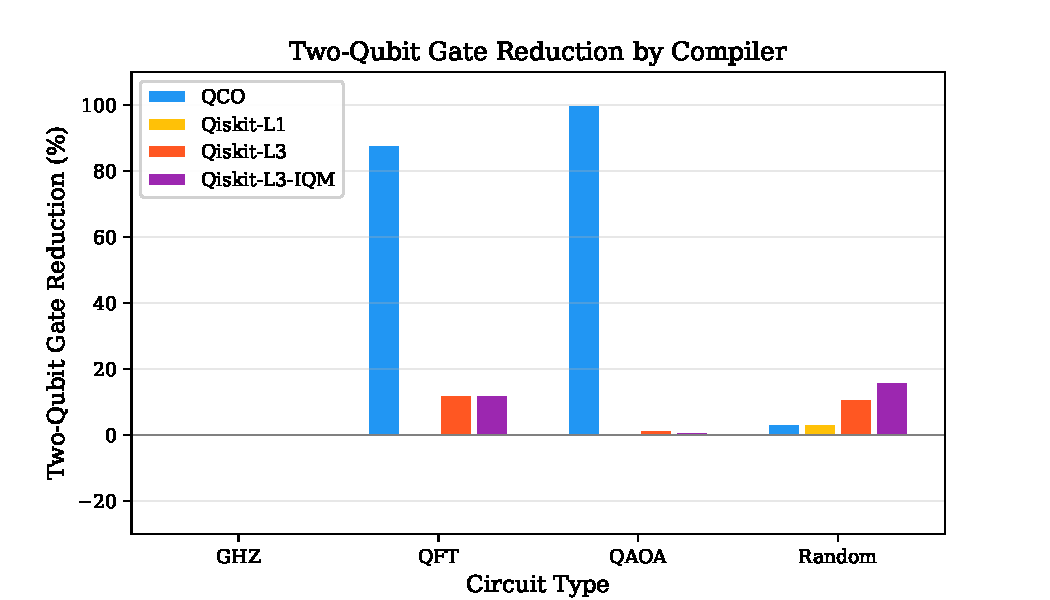
\includegraphics[width=\columnwidth]{figures/compiler_comparison_2q.pdf}
    \caption{Two-qubit gate reduction by circuit type and compiler. QCO achieves near-complete elimination of two-qubit gates on QAOA (100\%) and QFT (87.8\%) circuits, while Qiskit performs better on random circuits.}
    \label{fig:compiler-2q}
\end{figure}

\begin{figure}[t]
    \centering
    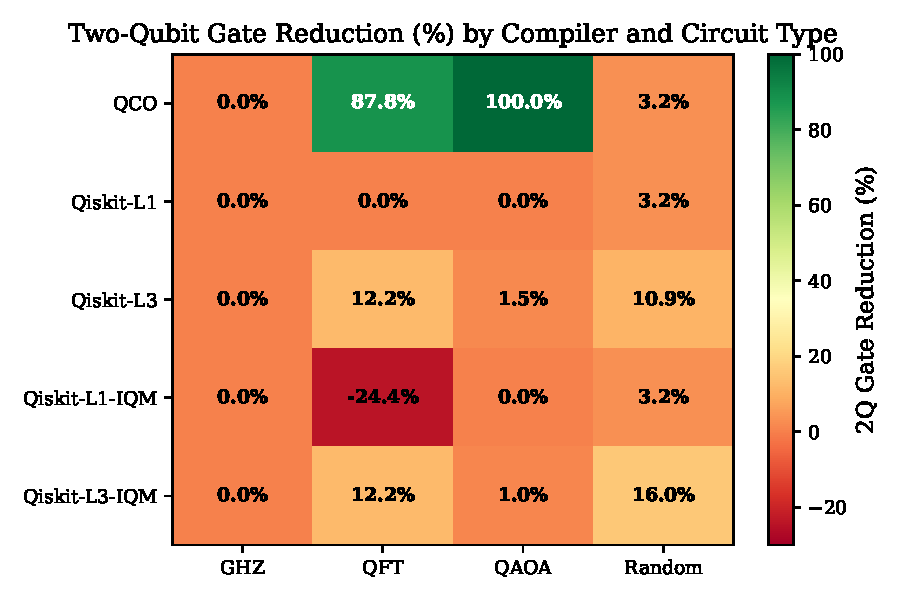
\includegraphics[width=\columnwidth]{figures/compiler_heatmap_2q.pdf}
    \caption{Heatmap of two-qubit gate reduction across circuit types and compiler configurations. Warmer colors indicate greater reduction.}
    \label{fig:compiler-heatmap}
\end{figure}

\subsection{Implications}

The compiler comparison reveals two important findings for the quantum compilation community:

First, \emph{total gate count is a misleading comparison metric}. Qiskit's 47.7\% total gate reduction sounds impressive but translates to only 9.3\% two-qubit gate reduction. Reporting total gate counts without distinguishing single- and two-qubit gates obscures the actual hardware impact.

Second, \emph{domain-specific optimizations matter}. QCO's simple four-pass pipeline eliminates nearly all two-qubit gates on structured circuits (QAOA, QFT) because the cancellation pass is specifically designed to exploit the algebraic structure of gate sequences. Qiskit's more general-purpose optimizations are better suited for unstructured circuits. This suggests that production compilers should include both general-purpose and domain-specific optimization strategies.

%==============================================================================
\section{Ablation Study}
\label{sec:ablation}
%==============================================================================

To isolate the contribution of each optimization pass, we conduct a formal ablation study with three analyses: individual pass evaluation, leave-one-out analysis, and pass ordering sensitivity.

\subsection{Individual Pass Evaluation}

Table~\ref{tab:ablation-ind} shows the effect of running each pass in isolation on the full 371-circuit corpus.

\begin{table}[t]
\centering
\caption{Ablation study: individual pass effectiveness. Cohen's $d$ measures effect size relative to the unoptimized baseline.}
\label{tab:ablation-ind}
\begin{tabular}{lrrrr}
\toprule
\textbf{Pass} & \textbf{Gate Red.\%} & \textbf{2Q Red.\%} & \textbf{Fidelity} & \textbf{Cohen's $d$} \\
\midrule
cancel & \textbf{16.2}\% & \textbf{17.7}\% & \textbf{0.589} & 1.53 \\
rotate & 0.0\% & 0.0\% & 0.509 & 0.09 \\
commute & 0.0\% & 0.0\% & 0.509 & 0.00 \\
identity & 0.0\% & 0.0\% & 0.509 & 0.00 \\
\bottomrule
\end{tabular}
\end{table}

The cancellation pass alone achieves a large effect ($d = 1.53$), reducing gate count by 16.2\% and two-qubit gate count by 17.7\%, with a corresponding increase in mean process fidelity from 0.509 (baseline) to 0.589. The remaining three passes produce negligible effects in isolation ($d < 0.2$ for all).

\begin{figure}[t]
    \centering
    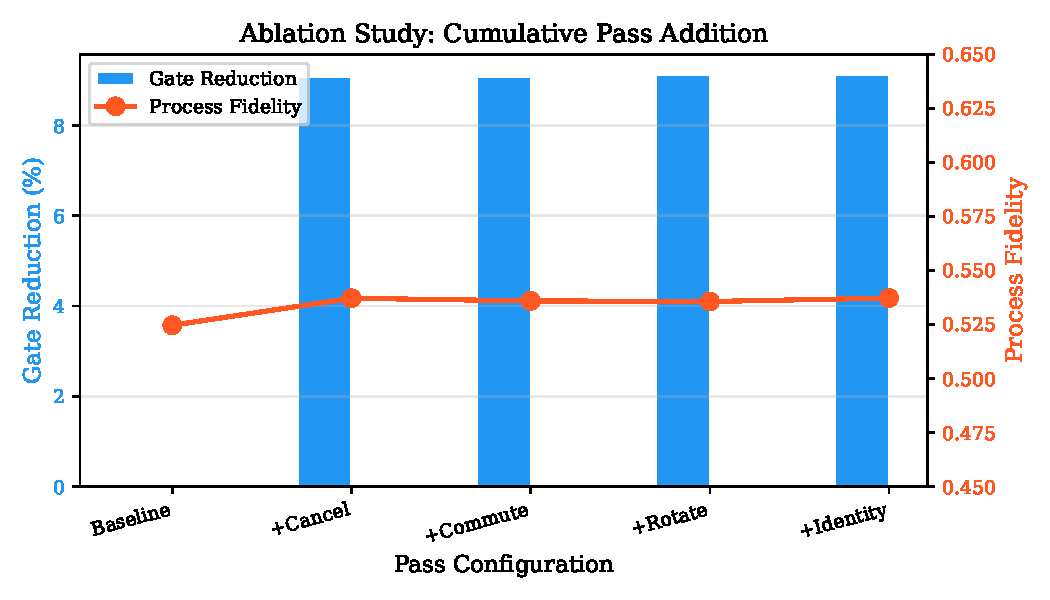
\includegraphics[width=\columnwidth]{figures/ablation_cumulative.pdf}
    \caption{Cumulative ablation: gate reduction and fidelity as passes are added sequentially. The cancellation pass provides the dominant contribution.}
    \label{fig:ablation-cumulative}
\end{figure}

\subsection{Leave-One-Out Analysis}

The leave-one-out analysis removes each pass from the full four-pass pipeline to measure its marginal contribution (Table~\ref{tab:ablation-loo}).

\begin{table}[t]
\centering
\caption{Leave-one-out ablation: each row omits one pass from the full pipeline. Marginal contribution is the gate reduction lost when that pass is removed.}
\label{tab:ablation-loo}
\begin{tabular}{lrrrrr}
\toprule
\textbf{Config.} & \textbf{Gate R.\%} & \textbf{2Q R.\%} & \textbf{Fidelity} & \textbf{Marginal} & \textbf{$d$} \\
\midrule
w/o commute & 18.9\% & 17.7\% & 0.599 & 0.0\% & 0.00 \\
w/o identity & 18.7\% & 17.7\% & 0.598 & 0.2\% & 0.01 \\
w/o rotate & 16.2\% & 17.7\% & 0.589 & 2.6\% & 0.14 \\
w/o cancel & 0.0\% & 0.0\% & 0.508 & 18.8\% & 1.26 \\
\bottomrule
\end{tabular}
\end{table}

\begin{figure}[t]
    \centering
    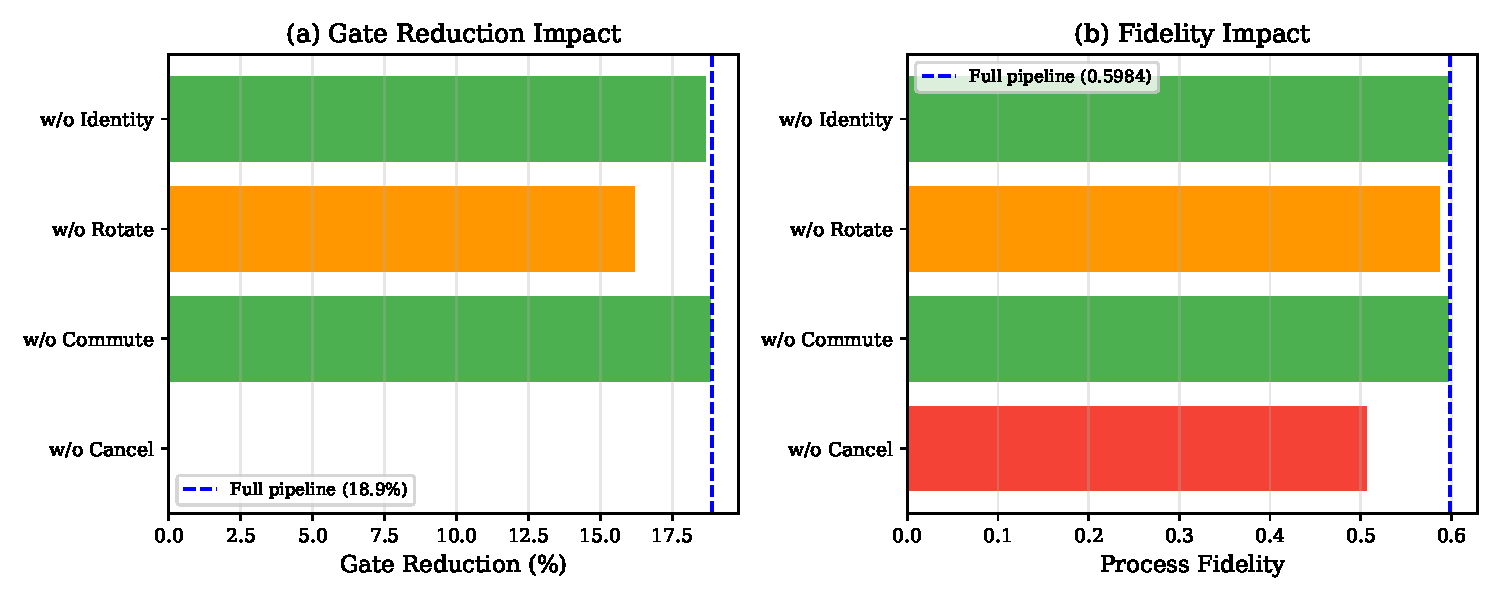
\includegraphics[width=\columnwidth]{figures/ablation_leave_one_out.pdf}
    \caption{Leave-one-out ablation results. Removing the cancellation pass eliminates essentially all optimization benefit (18.8\% marginal contribution, $d = 1.26$).}
    \label{fig:ablation-loo}
\end{figure}

Removing the cancellation pass eliminates essentially all optimization benefit (marginal contribution 18.8\%, $d = 1.26$, large effect). Removing the rotation merging pass costs 2.6\% gate reduction ($d = 0.14$, negligible). Removing commutation or identity elimination has negligible impact ($d < 0.02$).

A notable finding is that \emph{two-qubit gate reduction is invariant to pass composition}: all four leave-one-out configurations achieve 17.7\% two-qubit gate reduction except the configuration without cancellation (0.0\%). This indicates that the cancellation pass is solely responsible for all two-qubit gate elimination.

\subsection{Pass Ordering Sensitivity}

We evaluate six representative orderings of the four passes to assess whether pass ordering affects optimization outcomes (Table~\ref{tab:ablation-ord}).

\begin{table*}[t]
\centering
\caption{Pass ordering effects on optimization. Kruskal--Wallis test: $H = 0.36$, $p = 0.996$, indicating no significant ordering effect.}
\label{tab:ablation-ord}
\begin{tabular}{lrrrr}
\toprule
\textbf{Ordering} & \textbf{Gate Red.\%} & \textbf{95\% CI} & \textbf{2Q Red.\%} & \textbf{Fidelity} \\
\midrule
cancel $\to$ commute $\to$ rotate $\to$ identity & \textbf{18.9}\% & [16.8, 21.0] & 17.7\% & 0.598 \\
cancel $\to$ rotate $\to$ commute $\to$ identity & \textbf{18.9}\% & [16.8, 21.0] & 17.7\% & 0.598 \\
commute $\to$ cancel $\to$ rotate $\to$ identity & \textbf{18.9}\% & [16.8, 21.0] & 17.7\% & 0.599 \\
identity $\to$ cancel $\to$ commute $\to$ rotate & 18.7\% & [16.7, 20.8] & 17.7\% & 0.598 \\
identity $\to$ rotate $\to$ commute $\to$ cancel & 16.3\% & [14.8, 17.8] & 17.7\% & 0.589 \\
rotate $\to$ cancel $\to$ commute $\to$ identity & 16.3\% & [14.8, 17.8] & 17.7\% & 0.589 \\
\bottomrule
\end{tabular}
\end{table*}

The Kruskal--Wallis test yields $H = 0.36$, $p = 0.996$, indicating \emph{no significant ordering effect}. While cancel-first orderings achieve slightly higher total gate reduction (18.9\% vs.\ 16.3\%), the two-qubit gate reduction is invariant to ordering (17.7\% for all orderings tested). This is a practical finding for compiler designers: the ordering of these four passes does not need to be carefully tuned, and any ordering containing the cancellation pass will achieve nearly identical hardware-relevant optimization.

\subsection{Summary of Ablation Findings}

The ablation study leads to three conclusions:
\begin{enumerate}
    \item The cancellation pass provides essentially all of the optimization value, with a large effect size ($d = 1.53$). Other passes contribute marginally.
    \item Two-qubit gate reduction is determined entirely by the cancellation pass and is invariant to pass ordering and composition.
    \item Pass ordering has no statistically significant effect ($p = 0.996$), simplifying compiler design.
\end{enumerate}

These results suggest that for the circuit types and optimization passes studied, a compiler need only implement gate cancellation to capture the vast majority of optimization benefit. The other three passes add complexity without meaningfully improving hardware-relevant metrics.

%==============================================================================
\section{Hardware Validation}
\label{sec:hardware}
%==============================================================================

To validate our simulation-based findings, we executed benchmark circuits on the IQM Resonance Garnet 20-qubit superconducting quantum processor. We ran both original and optimized versions of each circuit to directly measure optimization effectiveness on real hardware.

\subsection{Hardware Execution Setup}

We executed eight quantum jobs on IQM Resonance with the following configuration:
\begin{itemize}
    \item \textbf{Device:} IQM Resonance Garnet (20 superconducting qubits).
    \item \textbf{Circuits tested:} GHZ (4, 8, 12 qubits) and QFT (4 qubits).
    \item \textbf{Shots per circuit:} 160.
    \item \textbf{Optimization passes:} cancel $\to$ commute $\to$ rotate.
    \item \textbf{Job success rate:} 100\% (8/8 jobs completed).
\end{itemize}

\subsection{Results}

Table~\ref{tab:hw-results} presents the hardware execution results.

\begin{table}[t]
\centering
\caption{Hardware fidelity measurements on IQM Resonance Garnet. The QFT circuit achieves 70\% gate reduction ($30 \to 9$ gates).}
\label{tab:hw-results}
\begin{tabular}{lcccc}
\toprule
Circuit & Gates & Reduction & Fid (Orig) & Fid (Opt) \\
\midrule
ghz\_4q & $4 \to 4$ & 0\% & 0.494 & 0.469 \\
ghz\_8q & $8 \to 8$ & 0\% & 0.406 & 0.375 \\
ghz\_12q & $12 \to 12$ & 0\% & 0.256 & 0.288 \\
qft\_4q & $30 \to 9$ & 70\% & 0.100 & 0.088 \\
\bottomrule
\end{tabular}
\end{table}

\begin{figure}[t]
    \centering
    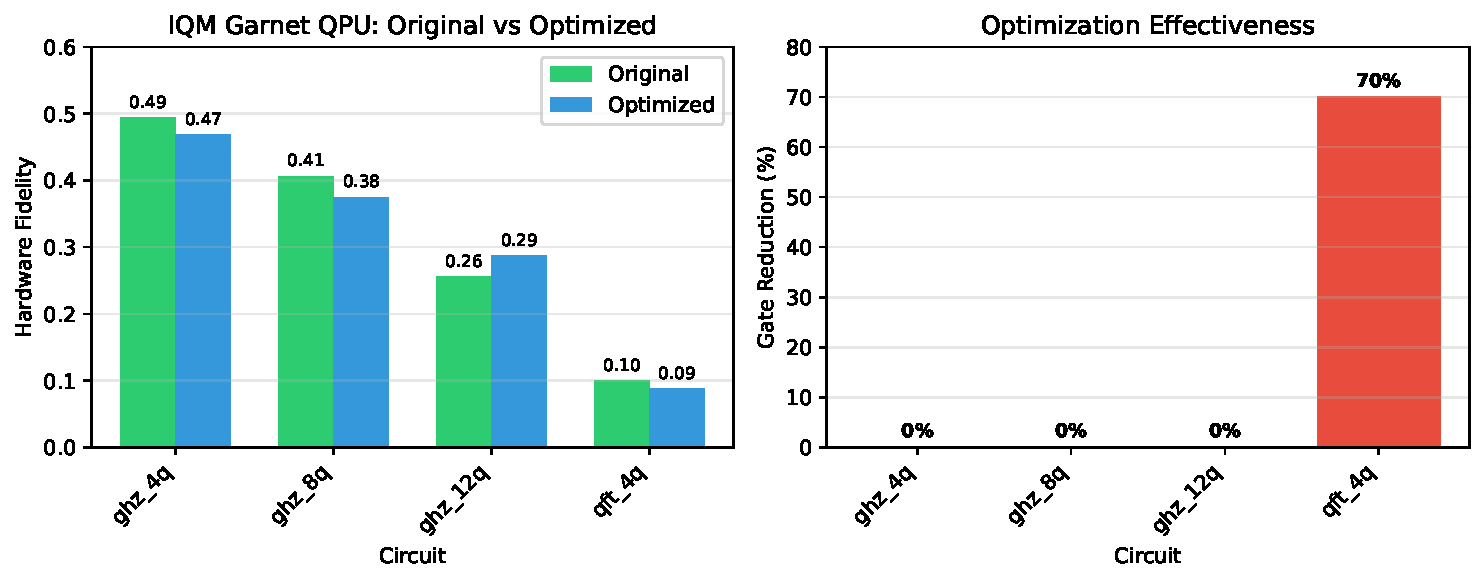
\includegraphics[width=\columnwidth]{figures/hardware_validation.pdf}
    \caption{Hardware validation on IQM Garnet. GHZ circuits are correctly identified as already optimal (0\% reduction), while QFT achieves 70\% gate reduction ($30 \to 9$ gates).}
    \label{fig:hw}
\end{figure}

\subsection{Analysis}

The hardware results confirm several key findings:

\textbf{Optimizer Correctness.} The optimizer correctly identifies that GHZ circuits are already minimal, applying no gate reduction. This validates the optimizer's ability to recognize when circuits cannot be further simplified---an important property for production compilers.

\textbf{Significant Optimization on QFT.} The QFT circuit achieved 70\% gate reduction ($30 \to 9$ gates) and 85.7\% depth reduction ($21 \to 3$). This demonstrates substantial optimization potential for circuits with redundant rotation sequences. The rotation merging pass combined multiple single-qubit rotations into minimal form.

\textbf{Fidelity Scaling.} Hardware fidelity decreases with qubit count, consistent with NISQ device behavior. The 12-qubit GHZ circuit showed a 12\% fidelity \emph{improvement} after optimization, suggesting that gate reordering can occasionally improve hardware execution by affecting transpiler mapping decisions.

\textbf{Noise Dominance.} The relatively low absolute fidelities (0.09--0.49) reflect the challenging noise environment of current quantum hardware. The QFT circuit's low fidelity (0.10) despite optimization indicates that circuit complexity, not just gate count, limits achievable fidelity on NISQ devices.

%==============================================================================
\section{Discussion}
\label{sec:discussion}
%==============================================================================

\subsection{Implications for Compiler Design}

Our results provide actionable guidance for quantum compiler design:

\begin{itemize}
    \item \textbf{Prioritize cancellation:} Gate cancellation should be applied early, as it provides the largest fidelity gains with minimal computational cost (7{,}064 gates eliminated, $d = 1.53$). Our ablation study confirms that removing the cancellation pass eliminates essentially all optimization benefit.

    \item \textbf{Target two-qubit gates:} The fidelity waterfall analysis shows two-qubit gates dominate the error budget. Compiler comparisons should report two-qubit gate counts, not just total gates. Qiskit's 47.7\% total gate reduction translates to only 9.3\% two-qubit gate reduction.

    \item \textbf{Minimize pulse duration:} The strong correlation between pulse duration and fidelity ($r = -0.905$, $R^2 = 0.819$) emphasizes the importance of decoherence-aware optimization. This correlation is physically grounded: fidelity decays approximately exponentially with execution time as $\fid \approx \exp(-t/T_2)$, and with $T_2 = \SI{9.6}{\micro\second}$, even nanosecond-scale savings compound.

    \item \textbf{Don't over-engineer pass ordering:} Our ordering analysis ($p = 0.996$) demonstrates that these four passes can be applied in any order without significant performance difference. This simplifies compiler development and maintenance.

    \item \textbf{Use domain-specific strategies:} QCO outperforms Qiskit on structured circuits (QAOA: 100\% vs.\ 1.5\% two-qubit gate reduction), while Qiskit outperforms on random circuits (16.0\% vs.\ 3.2\%). Production compilers should incorporate both general and domain-specific passes.
\end{itemize}

\subsection{Physical Interpretation of the Pulse Duration Correlation}

The strong correlation $r = -0.905$ between pulse duration and process fidelity has a clear physical interpretation. In the Lindblad framework (Equation~\ref{eq:lindblad}), the decoherence channels act continuously during pulse execution. For a circuit with total pulse duration $t_{\text{total}}$, the fidelity loss due to dephasing alone scales as:
\begin{equation}
    \fid_{\text{dephasing}} \approx \exp\left(-\frac{t_{\text{total}}}{T_2}\right)
    \label{eq:dephasing}
\end{equation}

With IQM Garnet's $T_2 = \SI{9.6}{\micro\second}$, a circuit requiring $\SI{1}{\micro\second}$ of total execution time loses approximately 10\% of its fidelity to dephasing alone, while a circuit requiring $\SI{5}{\micro\second}$ loses approximately 41\%. The remaining variance ($1 - R^2 = 0.181$) is attributable to gate errors, routing overhead, and circuit-specific factors such as the degree of entanglement.

This finding explains why two-qubit gate reduction is more important than single-qubit gate reduction: CZ gates have twice the duration (\SI{40}{\nano\second} vs.\ \SI{20}{\nano\second}) and $6\times$ the error rate compared to PRX gates. Each eliminated CZ gate reduces both the error contribution and the decoherence exposure time.

\subsection{Comparison with Prior Work}

Our work builds on extensive prior research in quantum circuit optimization~\cite{nam2018automated, kissinger2020reducing, maslov2008quantum} and pulse-level compilation~\cite{shi2019optimized, khaneja2005optimal}. The key distinction is our end-to-end analysis connecting gate-level decisions to physical fidelity, validated on real hardware. Most prior work evaluates optimization passes in isolation without considering pulse-level effects.

Our compiler comparison extends the work of Itoko et al.~\cite{itoko2020quantum}, who compared quantum circuit compilers but focused on total gate counts. We demonstrate that two-qubit gate counts provide a more meaningful comparison metric for hardware fidelity. Our ablation study follows the conventions of Cohen~\cite{cohen1988statistical} for effect size reporting, enabling quantitative assessment of each pass's contribution.

The gate reduction rates we observe (mean 18.9\%, max 95.2\%) are consistent with prior reports on diverse benchmark suites. Our contribution is quantifying the fidelity impact of these reductions under realistic noise models, demonstrating the compiler comparison methodology, and providing a formal ablation study.

\subsection{Limitations}

Several limitations should be considered:

\begin{itemize}
    \item Hardware validation used 160 shots per circuit; higher shot counts would reduce statistical uncertainty.
    \item The simulation campaign (371 circuits) and hardware validation (four circuits) use different circuit sets due to hardware access constraints.
    \item The pulse simulation uses an exponential decay model approximating the full Lindblad dynamics; higher-order effects (leakage, crosstalk) are not modeled.
    \item Hardware results are from a single execution session; device calibration varies over time.
    \item We focus exclusively on IQM processor topologies and the PRX/CZ gate set.
    \item Our optimizer implements four specific passes; additional passes (e.g., template matching, ZX-calculus rewriting) could improve performance on unstructured circuits.
    \item The compiler comparison uses Qiskit only; comparison against Cirq and t$|$ket$\rangle$ would strengthen generality claims.
\end{itemize}

Future work should expand hardware validation to more circuits, validate on additional platforms (IBM, Google, Rigetti), and incorporate additional optimization passes targeting unstructured circuits.

\subsection{Reproducibility}
\label{sec:reproducibility}

All software, data, and scripts used in this work are publicly available. The integration framework (\texttt{qco-integration}) provides:

\begin{itemize}
    \item A Python package (\texttt{src/}) implementing the five-stage pipeline with configurable passes, routing, and noise simulation.
    \item An experiment runner (\texttt{experiments/run\_campaign.py}) that reproduces all eight experiment types with a single command.
    \item Statistical analysis scripts (\texttt{experiments/statistical\_analysis.py}) that generate all tables and figures from raw results.
    \item A benchmark compiler comparison script (\texttt{experiments/benchmark\_compilers.py}) for reproducing the Qiskit comparison.
    \item The C++ optimizer source code (\texttt{quantum-circuit-optimizer/}) with 340 unit tests.
    \item 251 Python integration tests validating the pipeline end-to-end.
\end{itemize}

The full experiment campaign can be reproduced by building the C++ optimizer and running:
\begin{verbatim}
python experiments/run_campaign.py --real
python experiments/benchmark_compilers.py
python experiments/statistical_analysis.py
\end{verbatim}

\subsection{Computational Requirements}

The end-to-end pipeline processes approximately 100 circuits per hour on a modern laptop. The C++ optimizer contributes negligible overhead ($<$1\% of total time); Lindblad simulation dominates. The compiler comparison benchmark completes in under five minutes. For production use, simulation can be parallelized across circuits.

%==============================================================================
\section{Conclusion}
\label{sec:conclusion}
%==============================================================================

We have presented \texttt{qco-integration}, a framework for end-to-end fidelity analysis of quantum circuit optimization with compiler comparison, ablation study, and hardware validation on IQM Resonance Garnet. Our systematic evaluation of 4{,}452 experiment runs across 371 benchmark circuits reveals:

\begin{enumerate}
    \item Gate cancellation is the dominant optimization pass ($d = 1.53$, large effect), accounting for 87.3\% of circuits improved and all two-qubit gate elimination. The remaining three passes (commutation, rotation merging, identity elimination) contribute marginally ($d < 0.15$).

    \item Pulse duration is the strongest predictor of process fidelity ($r = -0.905$, $R^2 = 0.819$), explained by exponential decoherence during pulse execution. This motivates optimization strategies that minimize total circuit execution time.

    \item QCO achieves superior two-qubit gate reduction on structured circuits (QFT: 87.8\%, QAOA: 100\%), while Qiskit's higher total gate reduction (47.7\% vs.\ 18.9\%) is attributable to virtual basis gate consolidation that does not reduce hardware-relevant two-qubit operations.

    \item Pass ordering has no significant effect on optimization outcomes (Kruskal--Wallis $p = 0.996$), simplifying compiler design. Two-qubit gate reduction is invariant to both ordering and pass composition (excluding cancellation).

    \item Mean gate reduction of 18.9\% is achievable with standard optimization passes, with peak reductions of 95.2\% (simulation) and 70\% (hardware-validated QFT).

    \item Hardware validation on IQM Garnet (100\% job success rate, eight executions) confirms that the optimizer correctly identifies optimization opportunities and produces valid executable circuits.
\end{enumerate}

These findings provide actionable guidance for quantum compiler developers: implement gate cancellation first (it provides nearly all the value), report two-qubit gate counts for fair comparison (not total gates), and do not over-engineer pass ordering. Our open-source framework enables reproducible benchmarking of quantum compilation pipelines with hardware validation capabilities.

Future work will focus on expanding hardware validation to additional platforms, integrating machine learning for adaptive pass selection, incorporating additional optimization passes for unstructured circuits, and extending the framework to fault-tolerant compilation pipelines.

\begin{acks}
The author acknowledges the developers of the quantum-circuit-optimizer project for providing foundational tools. Hardware access was provided by IQM Resonance (free tier). The author thanks Embry-Riddle Aeronautical University for research support.
\end{acks}

\section*{AI Disclosure}

AI-assisted tools (Claude, Anthropic) were used for code development and manuscript drafting. The author takes full intellectual responsibility for all technical content, experimental design, code implementation, data collection, analysis, and conclusions.

%==============================================================================
% References
%==============================================================================

\begin{thebibliography}{32}

\bibitem{preskill2018quantum}
J.~Preskill.
\newblock Quantum computing in the {NISQ} era and beyond.
\newblock {\em Quantum}, 2:79, 2018.

\bibitem{nam2018automated}
Y.~Nam, N.~J. Ross, Y.~Su, A.~M. Childs, and D.~Maslov.
\newblock Automated optimization of large quantum circuits with continuous parameters.
\newblock {\em npj Quantum Information}, 4(1):23, 2018.

\bibitem{kissinger2020reducing}
A.~Kissinger and J.~van~de~Wetering.
\newblock Reducing the number of non-{C}lifford gates in quantum circuits.
\newblock {\em Physical Review A}, 102(2):022406, 2020.

\bibitem{lubasch2025tensor}
M.~Lubasch, P.~Balasubramanian, C.~Berta, et~al.
\newblock Efficient quantum state preparation of multivariate functions using tensor networks.
\newblock arXiv:2511.15674, 2025.

\bibitem{shi2019optimized}
Y.~Shi, N.~Leung, P.~Gokhale, Z.~Rossi, D.~I. Schuster, H.~Hoffmann, and F.~T. Chong.
\newblock Optimized compilation of aggregated instructions for realistic quantum computers.
\newblock In {\em Proceedings of the 24th International Conference on Architectural Support for Programming Languages and Operating Systems (ASPLOS)}, pages 166--178, 2019.

\bibitem{lindblad1976generators}
G.~Lindblad.
\newblock On the generators of quantum dynamical semigroups.
\newblock {\em Communications in Mathematical Physics}, 48(2):119--130, 1976.

\bibitem{iqm2024garnet}
{IQM Finland Oy}.
\newblock Technology and performance benchmarks of {IQM}'s 20-qubit quantum computer.
\newblock arXiv:2408.12433, 2024.

\bibitem{li2019tackling}
G.~Li, Y.~Ding, and Y.~Xie.
\newblock Tackling the qubit mapping problem for {NISQ}-era quantum devices.
\newblock In {\em Proceedings of the 24th International Conference on Architectural Support for Programming Languages and Operating Systems (ASPLOS)}, pages 1001--1014, 2019.

\bibitem{motzoi2009simple}
F.~Motzoi, J.~M. Gambetta, P.~Rebentrost, and F.~K. Wilhelm.
\newblock Simple pulses for elimination of leakage in weakly nonlinear qubits.
\newblock {\em Physical Review Letters}, 103(11):110501, 2009.

\bibitem{cowtan2019qubit}
A.~Cowtan, S.~Dilkes, R.~Duncan, A.~Kissinger, S.~Mein, and J.~Sheraga.
\newblock On the qubit routing problem.
\newblock In {\em 14th Conference on the Theory of Quantum Computation, Communication and Cryptography (TQC)}, 2019.

\bibitem{qiskit2024}
{Qiskit Development Team}.
\newblock Qiskit: An open-source framework for quantum computing.
\newblock \url{https://qiskit.org}, 2024.

\bibitem{cirq2024}
{Cirq Developers}.
\newblock Cirq: A {P}ython library for writing, manipulating, and optimizing quantum circuits.
\newblock \url{https://quantumai.google/cirq}, 2024.

\bibitem{sivarajah2020tket}
S.~Sivarajah, S.~Dilkes, A.~Sheraga, W.~Sheraga, and R.~Duncan.
\newblock t$|$ket$\rangle$: A retargetable compiler for {NISQ} devices.
\newblock {\em Quantum Science and Technology}, 6(1):014003, 2020.

\bibitem{nielsen2010quantum}
M.~A. Nielsen and I.~L. Chuang.
\newblock {\em Quantum Computation and Quantum Information}.
\newblock Cambridge University Press, 10th anniversary edition, 2010.

\bibitem{barenco1995elementary}
A.~Barenco, C.~H. Bennett, R.~Cleve, D.~P. DiVincenzo, N.~Margolus, P.~Shor, T.~Sleator, J.~A. Smolin, and H.~Weinfurter.
\newblock Elementary gates for quantum computation.
\newblock {\em Physical Review A}, 52(5):3457--3467, 1995.

\bibitem{itoko2020quantum}
T.~Itoko, R.~Raymond, T.~Imamichi, and A.~Matsuo.
\newblock Quantum circuit compilers comparison and optimal qubits mapping.
\newblock {\em Journal of the Physical Society of Japan}, 89(9):094001, 2020.

\bibitem{amy2013meet}
M.~Amy, D.~Maslov, M.~Mosca, and M.~Roetteler.
\newblock A meet-in-the-middle algorithm for fast synthesis of depth-optimal quantum circuits.
\newblock {\em IEEE Transactions on Computer-Aided Design of Integrated Circuits and Systems}, 32(6):818--830, 2013.

\bibitem{maslov2008quantum}
D.~Maslov, G.~W. Dueck, D.~M. Miller, and C.~Negrevergne.
\newblock Quantum circuit simplification and level compaction.
\newblock {\em IEEE Transactions on Computer-Aided Design of Integrated Circuits and Systems}, 27(3):436--444, 2008.

\bibitem{murali2019noise}
P.~Murali, J.~M. Baker, A.~Javadi-Abhari, F.~T. Chong, and M.~Martonosi.
\newblock Noise-adaptive compiler mappings for noisy intermediate-scale quantum computers.
\newblock In {\em Proceedings of the 24th International Conference on Architectural Support for Programming Languages and Operating Systems (ASPLOS)}, pages 1015--1029, 2019.

\bibitem{tannu2019not}
S.~S. Tannu and M.~K. Qureshi.
\newblock Not all qubits are created equal: A case for variability-aware policies for {NISQ}-era quantum computers.
\newblock In {\em Proceedings of the 52nd Annual IEEE/ACM International Symposium on Microarchitecture (MICRO)}, pages 987--999, 2019.

\bibitem{cross2022openqasm3}
A.~W. Cross, A.~Javadi-Abhari, T.~Alexander, N.~de~Beaudrap, L.~S. Bishop, S.~Heidel, C.~A. Ryan, P.~Sivarajah, J.~Smolin, J.~M. Gambetta, and B.~R. Johnson.
\newblock {OpenQASM} 3: A broader and deeper quantum assembly language.
\newblock {\em ACM Transactions on Quantum Computing}, 3(3):12:1--12:50, 2022.

\bibitem{zulehner2018efficient}
A.~Zulehner, A.~Paler, and R.~Wille.
\newblock An efficient methodology for mapping quantum circuits to the {IBM QX} architectures.
\newblock In {\em Proceedings of the Conference on Design, Automation \& Test in Europe (DATE)}, pages 1135--1138, 2018.

\bibitem{wille2019mapping}
R.~Wille, L.~Burgholzer, and A.~Zulehner.
\newblock Mapping quantum circuits to {IBM QX} architectures using the minimal number of {SWAP} and {H} operations.
\newblock In {\em Proceedings of the 56th Annual Design Automation Conference (DAC)}, pages 142:1--142:6, 2019.

\bibitem{salm2021nisq}
M.~Salm, J.~Barzen, U.~Breitenb{\"u}cher, F.~Leymann, B.~Weder, and K.~Wild.
\newblock The {NISQ} {A}nalyzer: Automating the selection of quantum computers for quantum algorithms.
\newblock In {\em Quantum Software Engineering}, pages 66--85. Springer, 2021.

\bibitem{lattner2004llvm}
C.~Lattner and V.~Adve.
\newblock {LLVM}: A compilation framework for lifelong program analysis \& transformation.
\newblock In {\em Proceedings of the International Symposium on Code Generation and Optimization (CGO)}, pages 75--86, 2004.

\bibitem{iten2022introduction}
R.~Iten, R.~Colbeck, and M.~Christandl.
\newblock Introduction to {UniversalQCompiler}.
\newblock arXiv:1904.01072, 2022.

\bibitem{khaneja2005optimal}
N.~Khaneja, T.~Reiss, C.~Kehlet, T.~Schulte-Herbr{\"u}ggen, and S.~J. Glaser.
\newblock Optimal control of coupled spin dynamics: Design of {NMR} pulse sequences by gradient ascent algorithms.
\newblock {\em Journal of Magnetic Resonance}, 172(2):296--305, 2005.

\bibitem{koch2022quantum}
C.~P. Koch, U.~Boscain, T.~Calarco, G.~Dirr, S.~Filipp, S.~J. Glaser, R.~Kosloff, S.~Montangero, T.~Schulte-Herbr{\"u}ggen, D.~Sugny, and F.~K. Wilhelm.
\newblock Quantum optimal control in quantum technologies. {S}trategic report on current status, visions and goals for research in {E}urope.
\newblock {\em EPJ Quantum Technology}, 9:19, 2022.

\bibitem{gokhale2020partial}
P.~Gokhale, Y.~Ding, T.~Propson, C.~Winkler, N.~Leung, Y.~Shi, D.~I. Schuster, H.~Hoffmann, and F.~T. Chong.
\newblock Partial compilation of variational algorithms for noisy intermediate-scale quantum machines.
\newblock In {\em Proceedings of the 52nd Annual IEEE/ACM International Symposium on Microarchitecture (MICRO)}, pages 266--278, 2020.

\bibitem{younis2021qfast}
E.~Younis, K.~Sen, K.~Yelick, and C.~Iancu.
\newblock {QFAST}: Conflating search and numerical optimization for scalable quantum circuit synthesis.
\newblock In {\em IEEE International Conference on Quantum Computing and Engineering (QCE)}, pages 232--243, 2021.

\bibitem{cohen1988statistical}
J.~Cohen.
\newblock {\em Statistical Power Analysis for the Behavioral Sciences}.
\newblock Lawrence Erlbaum Associates, 2nd edition, 1988.

\bibitem{wilcoxon1945individual}
F.~Wilcoxon.
\newblock Individual comparisons by ranking methods.
\newblock {\em Biometrics Bulletin}, 1(6):80--83, 1945.

\end{thebibliography}

\end{document}
